\documentclass{standalone}
\RequirePackage[table]{xcolor}
\RequirePackage{colortbl}
\RequirePackage{mhchem}
% Chapters
\definecolor{IBcolCH01}{HTML}{eb3b79}\colorlet{IBcolCH1}{IBcolCH01}
\definecolor{IBcolCH02}{HTML}{9a529f}\colorlet{IBcolCH2}{IBcolCH02}
\definecolor{IBcolCH03}{HTML}{775ba6}\colorlet{IBcolCH3}{IBcolCH03}
\definecolor{IBcolCH04}{HTML}{5a68b0}\colorlet{IBcolCH4}{IBcolCH04}
\definecolor{IBcolCH05}{HTML}{55a0d8}\colorlet{IBcolCH5}{IBcolCH05}
\definecolor{IBcolCH06}{HTML}{34b0e5}\colorlet{IBcolCH6}{IBcolCH06}
\definecolor{IBcolCH07}{HTML}{34c1d7}\colorlet{IBcolCH7}{IBcolCH07}
\definecolor{IBcolCH08}{HTML}{65bc6a}\colorlet{IBcolCH8}{IBcolCH08}
\definecolor{IBcolCH09}{HTML}{9acb62}\colorlet{IBcolCH9}{IBcolCH09}
\definecolor{IBcolCH10}{HTML}{d1dd5b}
\definecolor{IBcolCH11}{HTML}{f9ec5d}
\definecolor{IBcolCH12}{HTML}{fbc82a}
\definecolor{IBcolCH13}{HTML}{faa725}
\definecolor{IBcolCH14}{HTML}{f26f47}
\definecolor{IBcolCH15}{HTML}{8e6d65}
\definecolor{IBcolCH16}{HTML}{bdbcbc}
\definecolor{IBcolCH17}{HTML}{79919d}
% Learning/definition color
\definecolor{IBcolDef}{HTML}{ef5052}
% Step by step color
\definecolor{IBcolSBS}{HTML}{26a69b}
% Example box color
\definecolor{IBcolEXB}{HTML}{26a69b}
% Cover page
\definecolor{IBcolCOV}{HTML}{073f5c}
\definecolor{IBcolCOV2}{HTML}{3b4d72}
\definecolor{IBcolCOV3}{HTML}{fad155}
\definecolor{IBcolCOV4}{HTML}{1b3b5a}
% Chemistry
\definecolor{IBcolV}{HTML}{26a65b}
\definecolor{IBcolX}{HTML}{a62631}
\usepackage{tikz}
\usetikzlibrary{arrows.meta,decorations.markings,angles,quotes,snakes,plotmarks,3d}
\begin{document}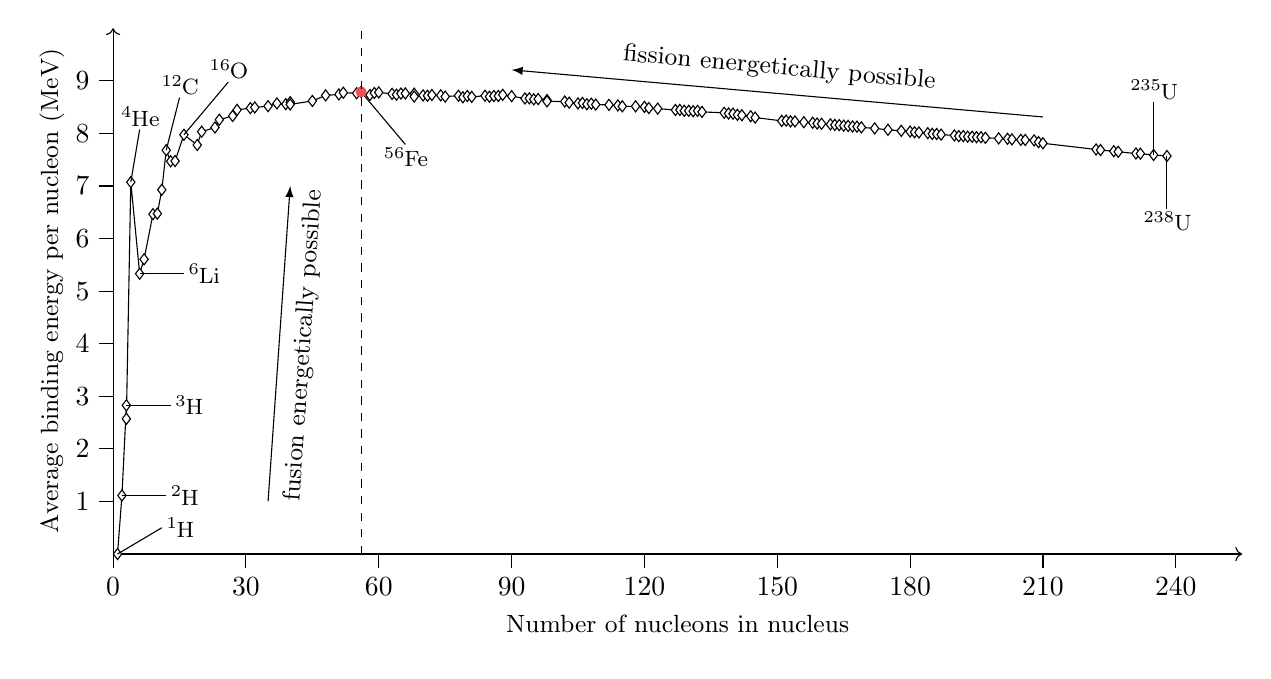
\begin{tikzpicture}[x=1.6pt,y=19pt]
    \draw[->] (0,0) -- (255,0);
    \node[below] at ({255/2},-17pt) {\small\strut Number of nucleons in nucleus};
    \draw[->] (0,0) -- (0,10);
    \node[above,rotate=90] at (-13pt,5) {\small\strut Average binding energy per nucleon (MeV)};
    \foreach \x in {0,30,...,240} {\draw (\x,0)--++(270:5pt) node[at end,below] {\x};}
    \foreach \y in {1,2,...,9} {\draw (0,\y)--++(180:5pt) node[at end,left] {\y};}
    \draw[mark=diamond*,mark options={fill=white}] plot coordinates{
        (  1,0.000) (  2,1.113) (  3,2.828) (  3,2.572) (  4,7.073) (  6,5.331) (  7,5.606) (  9,6.463) ( 10,6.474) ( 11,6.927) ( 12,7.680) ( 13,7.469) ( 14,7.474) ( 16,7.974) ( 19,7.779) ( 20,8.032) ( 23,8.112) ( 24,8.260) ( 27,8.331) ( 28,8.447) ( 31,8.480) ( 32,8.493) ( 35,8.518) ( 37,8.570) ( 39,8.557) ( 40,8.595) ( 40,8.551) ( 45,8.617) ( 48,8.722) ( 51,8.741) ( 52,8.774) ( 55,8.763) ( 56,8.790) ( 58,8.730) ( 59,8.768) ( 60,8.779) ( 63,8.752) ( 64,8.735) ( 65,8.757) ( 66,8.760) ( 68,8.755) ( 68,8.700) ( 70,8.722) ( 71,8.716) ( 72,8.730) ( 74,8.724) ( 75,8.700) ( 78,8.716) ( 79,8.686) ( 80,8.711) ( 81,8.694) ( 84,8.716) ( 85,8.697) ( 86,8.711) ( 87,8.711) ( 88,8.733) ( 90,8.708) ( 93,8.664) ( 94,8.667) ( 95,8.647) ( 96,8.653) ( 98,8.634) ( 98,8.609) (102,8.606) (103,8.584) (105,8.570) (106,8.579) (107,8.554) (108,8.565) (109,8.548) (112,8.543) (114,8.532) (115,8.515) (118,8.515) (120,8.504) (121,8.482) (123,8.471) (127,8.444) (128,8.447) (129,8.430) (130,8.430) (131,8.422) (132,8.428) (133,8.408) (138,8.392) (139,8.378) (140,8.375) (141,8.353) (142,8.345) (144,8.326) (145,8.301) (151,8.238) (152,8.243) (153,8.227) (154,8.227) (156,8.213) (158,8.202) (159,8.188) (160,8.183) (162,8.172) (163,8.161) (164,8.158) (165,8.147) (166,8.142) (167,8.131) (168,8.128) (169,8.114) (172,8.095) (175,8.068) (178,8.048) (180,8.035) (181,8.021) (182,8.018) (184,8.004) (185,7.991) (186,7.988) (187,7.977) (190,7.960) (191,7.947) (192,7.949) (193,7.938) (194,7.936) (195,7.927) (196,7.927) (197,7.916) (200,7.905) (202,7.897) (203,7.886) (205,7.878) (206,7.875) (208,7.867) (209,7.834) (210,7.812) (222,7.694) (223,7.683) (226,7.661) (227,7.650) (231,7.617) (232,7.614) (235,7.589) (238,7.570) };

    \begin{scope}[every node/.style={font=\footnotesize,inner sep=1pt}]
        \draw (1,0)      --++(10,0.5)   node[at end,right]{\ce{^1H}};
        \draw (2,1.113)  --++(10,0)   node[at end,right] {\ce{^2H}};
        %\draw (3,2.572)  --++(10,-0.5)   node[at end,right] {\ce{^3He}};
        \draw (3,2.828)  --++(10,0)   node[at end,right] {\ce{^3H}};
        \draw (6,5.331)  --++(10,0)  node[at end,right] {\ce{^6Li}};
        %\draw (7,5.606)  --++(10,0.5)   node[at end,right] {\ce{^7Li}};
        \draw (4,7.073)  --++(2,1)   node[at end,above] {\ce{^4He}};
        \draw (12,7.680)  --++(3,1)  node[at end,above] {\ce{^12C}};
        \draw (16,7.974)  --++(10,1)  node[at end,above] {\ce{^16O}};
        \draw (56,8.790)  --++(10,-1) node[at end,below] {\ce{^56Fe}};
        \fill[IBcolDef] (56,8.790) circle (2pt);
        \draw (235,7.589) --++(0,1)  node[at end,above] {\ce{^235U}};
        \draw (238,7.570) --++(0,-1) node[at end,below] {\ce{^238U}};
    \end{scope}
    \draw[dashed] (56,0) -- (56,10);
    \draw[-latex] (35,1) -- (40,7) node[midway,below,sloped] {\small\strut fusion energetically possible};
    \draw[-latex] (210,8.312) -- (90,9.208) node[midway,above,sloped] {\small\strut fission energetically possible};
\end{tikzpicture}\end{document}